\documentclass[a4paper,10pt]{article}
\usepackage{graphicx}

\title{Werkplan\\\small Software Engineering en Gedistribueerde Applicaties\\\small Team 8}
\author{Chris Bovenschen,Harm Dermois, Alexandra Pizarro, Tamara Ockhuis \and Fredo Tan\\\small 6104096,0527963,6129544,6060374\and 6132421 }
\begin{document}
\maketitle
\tableofcontents
\section{Inleiding}
Dit is het werkplan van team FACHT voor het vak Software Enginering en Gedistribueerde
Applicaties. In dit document is de planning de deliverables,de modules, model en planning te vinden van ons project. De project leider is Harm Dermois. De secretarissen zijn ingedeeld als volgt:
\begin{itemize}
\item Week 1: Fredo
\item Week 2: Alexandra
\item Week 3: Tamara
\item Week 4: Chris
\end{itemize}
Het uiteindelijke doel is een robot te maken die zelf rond kan rijden en een map kan maken. Nadat er een map is gemaakt een pad kan plannen die je van punt a naar b brengt.
\section{Model}
De module listener is verbonden aan de server via een TCP connectie. Deze wordt tevens gebruikt om commando�s naar de robot te sturen. De onvangen comando's worden doorgegeven naar de sensormodulen die kijken of de data daadwerkelijk geldig is en binnen de parameters valt, zodat we de data van de robot kunnen gebruiken. We hebben drie sensormodules waar we informatie vandaan halen: sonar, laser en odometry. Vanuit deze laag gaat de data naar de laag waar de mid-level modules zich bevinden die dienen voor de muurzoeker en muurvolger. De data voor de module kaartenmaker komt rechtstreeks uit de sensormodules. Berekende kaarten uit de kaartenmaker kunnen gebruikt worden voor de routeplanner. De routeplanner geeft zijn berekende pad tenslotte door aan module bewegingen. De botsing ontwijker is een module die botsingen kan detecteren en aan de andere modules meld wanneer er een botsing zal gaan plaatsvinden.
We hebben gekozen voor dit model om het wat robuster te maken. Als de listener niet werkt het hele programma niet, maar als er 1 van de sensormodulen kan het programma
nog steeds blijven draaien. Ook hebben we het gedrag van de robot dus opgedeeld in 3 verschillende modules namelijk: muurzoeken, muurvolgen en de routeplanner. Van deze modules kan er maar 1 tegelijk aanstaan. 
%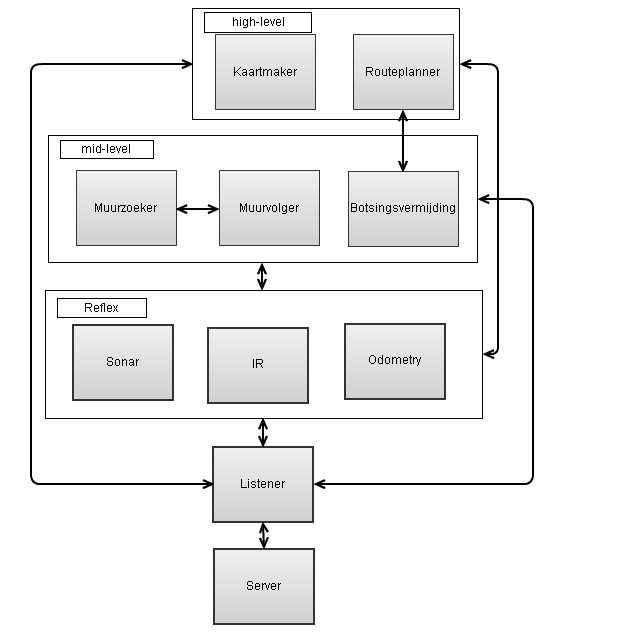
\includegraphics[scale = 0.5]{flowchart.PNG} plaatje
\section{Deliverables}
Het plan is om aan het eind van het project een robot te leveren die zich kan voortbewegen door middel van berekeningen die gebaseerd zijn op data afkomstig van de sensoren. Vervolgens is het de bedoeling dat de robot diens omgeving in kaart kan brengen met behulp van de informatie van de sensoren. De robot moet in staat zijn om:
in een vrij volle ruimte gevuld met diverse obstakels een pad langs een wand te kunnen afleggen.
Dus wij leveren de volgende modules:
\begin{enumerate}
\item De movements
\item Een listener.
\item Reflex/sensor modules per soort data.
\item Een muurzoeker.
\item Een muurvolger.
\item Een botsing vermijder.
\item Een routplanner.
\item Een mapmaker.
\item Een communicator die tussen modules kan praten.
\item Een werkend geheel die alle modules met elkaar combineert.
\end{enumerate}
Uitleg over de modules te vinden in section \ref{sec:modules}.
Bij de eerste deliverable leveren de volgende modules: De listener, de muurvolger, de muurzoeker, de reflex/sensor en communicator. Deze zijn allemaal standalone en maken hun eigen connectie met de server. De tweede deliverable is het eind product en hebben we een werkend geheel.
\section{Testen}
Alle modules hebben we apart getest. Elke module moet standalone kunnen werken en de verschillende We hebben elke module direct aan de aan de simulator vast gezet en met de echte data de modules getest. Wanneer we denken dat de modules werken gaan we ze verder testen op onconventionele omstandigheden. De pre-condities worden aan het begin
van de methode gedefineerd. Wanneer je in de module komt met waardes die niet voldoet aan de pre-condities worden genegeerd.
Al deze modules worden
later gemodificeerd met de communicator methode zodat ze met elkaar kunnen praten.

\section{Modules}
\label{sec:modules}
Alle geteste modules worden voorzien van een communicator. Deze communicator leest uit waar alle modules zich bevinden. Wanneer de communicator wordt opgestart wordt een
thread gestart die connecties kan aannemen. Deze thread start op zijn beurt nog een andere thread op die luistert naar alle inkomende request en handelt deze af. Het preciese protocol voor de communicatie moet nog nader bepaald worden. Onze definitie van een muur zijn alle obstakels die we zien. Wij gebruiken geen camera dus het moeilijk een verschil te maken tussen een muur een blok die in de weg staat.\\
precondities:
\subsection{Movement}
Dit is een bibliotheek waarin alle bewegingen in zijn gedefinieerd. Deze kan geimporteerd worden door alle modules die de robot willen veranderen.
\subsection{Listener}
De listener is de module die direct aan de server vast zit. Deze haalt de informatie binnen van die de robot opstuurt, maar stuurt ook commando's naar de robot. Dit maakt de commando's naar de robot in ieder geval consistent. De data die wordt ontvagen worden direct opgestuurd naar de respectievelijke reflex modules die de data dan verder bewerken. Er moeten misschien nog levels worden toegevoegd voor de urgency van de commando's.
\subsection{Reflex modules}
De reflex modules krijgen de respectievelijke data van de listener. Deze modules zijn een soort opslag plaats van voor de meest recente data die de listener heeft gekregen. Deze modules kunnen de robot ook stoppen wanneer de data die ze binnen krijgen niet binnen de verwachte parameters zijn. Daarom zijn het de reflex modules. Deze modules kunnen door de hogere level modules aangeroepen worden voor de meest recente data.
\subsection{Botsing ontwijker}
De botsing ontwijker wordt hoort bij de routeplanner module. Deze methode runt alleen wanneer de routeplanner aan het werken is. Deze detecteert dingen die niet op de map zit. dus de botsing ontwijker wordt alleen gebruikt voor dingen die onvoorzien zijn.
\subsection{Muurzoeker}
De muurzoeker is de mode waarin het zich bevindt wanneer de robot de wereld moet verkennen. De robot begint met om zich heen te kijken de kleinste waarde op te zoeken en daar heen te bewegen. Wanneer er een bepaalde drempelwaarde is bereikt gaan we ervan uit dat er een muur is gevonden en gaan we over naar de muurvolger module die dan verder gaat met de gevonden muur te volgen.
\subsection{Muurvolger}
De muurvolger volgt de muur die in de muurzoeker gevonden is. Hier draait het 90 graden zodat de kleinste waarde van de sonar in een van de buitenste sensoren te vinden is. Hierna blijft hij door gaan totdat er geen muur is om te volgen en gaat dan weer over naar de muurzoeker.
\subsection{Routeplanner}
De Routeplanner kan alleen gebruikt worden wanneer er al een map is gemaakt en kan dus alleen een route plannen binnen een bekend domein. Hierin probeert hij een zo kort mogelijk pad te vinden naar de bestemming. 
\subsection{Mapmaker}
De mapmaker krijgt een constante stroom van sonar en IR data waarmee hij dan een map gaat maken met waarschijnlijk wat uitbreidingen.
\section{Planning}
Er zijn vier weken beschikbaar voor dit project. In de eerste week van het project wordt de listener als eerst gerealiseerd. Daarnaast wordt de module die de methoden bevat voor de bewegingen geschreven. Wanneer dat gelukt is, maken we in dezelfde week nog een begin aan de sensormodules. De drie modules muurzoeker, muurvolger en botsingsvermijding zijn de volgende componenten die ge�mplementeerd moeten worden. Dat willen we graag in de tweede week doen. Wanneer dat voltooid is, maken we de �high level� componenten aan: de routeplanner en de kaartenmaker. We denken dat deze twee onderdelen vrij gecompliceerd zijn, hier willen we dan ruim de tijd voor nemen.

17 juni is de dag wanneer de eerste deliverable gereed moet zijn. Naar verwachting zal de eerste deliverable de listener, bewegingen en (een deel van) de �mid level� componenten omvatten. In de derde week vindt het inleveren van de tweede deliverable plaats. Op 23 juni willen we �mid level� componenten en de �high level� componenten gereed hebben.\\
Onze focus en deliverables per week.
\begin{tabular}{|l|p{5cm}|p{5cm}|}
\hline
Week&Focus&Deliverables\\
\hline
week 1&listener,bewegingen,sensor en werkplan& listener, beweging, sensoren en schetswerkplan \\ 
\hline
week 2&echte werkplan en mid-level modules en tests& werkplan en mid-level modules\\
\hline
week 3&mapmaking, routeplannen en tests & mapmaking\\
\hline
week 4& eindverslag, opschonen code testen& eind code en verslag\\
\hline

\end{tabular}

\end{document}